% define \title (only used by writelatex.com)
%\title{CSEC-793 Project Report_Blank}
%%%%%%%%%%%%%%%%%%%%%%%%%%%%%%%%%%%%%%%%%%%%%%%%%%%%%%%%%%%%%%%%%%%%%%
% LaTeX Template: Project Titlepage
%
% Source: http://www.howtotex.com
% Date: April 2011
% 
% This is a title page template which be used for articles & reports.
% 
% Feel free to distribute this example, but please keep the referral
% to howtotex.com
% 
%%%%%%%%%%%%%%%%%%%%%%%%%%%%%%%%%%%%%%%%%%%%%%%%%%%%%%%%%%%%%%%%%%%%%%
% How to use writeLaTeX: 
%
% You edit the source code here on the left, and the preview on the
% right shows you the result within a few seconds.
%
% Bookmark this page and share the URL with your co-authors. They can
% edit at the same time!
%
% You can upload figures, bibliographies, custom classes and
% styles using the files menu.
%
% If you're new to LaTeX, the wikibook is a great place to start:
% http://en.wikibooks.org/wiki/LaTeX
%
%%%%%%%%%%%%%%%%%%%%%%%%%%%%%%%%%%%%%%%%%%%%%%%%%%%%%%%%%%%%%%%%%%%%%%
%
% --------------------------------------------------------------------
% Preamble
% --------------------------------------------------------------------
\documentclass[ fontsize=11pt,twoside]{scrartcl}	% KOMA

\usepackage[letterpaper,pdftex]{geometry}	% A4paper margins
\setlength{\oddsidemargin}{5mm}			% Remove 'twosided' indentation
\setlength{\evensidemargin}{5mm}

\usepackage[english]{babel}
\usepackage[protrusion=true,expansion=true]{microtype}	
\usepackage{amsmath,amsfonts,amsthm,amssymb}
\usepackage{graphicx}
\usepackage{pseudocode}
\usepackage{siunitx}				% SI units

\usepackage[utf8]{inputenc}      % Use UTF-8 encoding
\usepackage[T1]{fontenc}         % Use modern font encoding
\usepackage{lmodern}             % Use scalable Latin Modern fonts
\usepackage{microtype}           % Enables font expansion
\usepackage{tikz}
\usepackage{float}
\usetikzlibrary{shapes,arrows}


% --------------------------------------------------------------------
% Definitions (do not change this)
% --------------------------------------------------------------------
\newcommand{\HRule}[1]{\rule{\linewidth}{#1}} 	% Horizontal rule

\makeatletter							% Title
\def\printtitle{%						
    {\centering \@title\par}}
\makeatother									

\makeatletter							% Author
\def\printauthor{%					
    {\centering \Large \@author}}				
\makeatother							

% --------------------------------------------------------------------
% Metadata (Change this)
% --------------------------------------------------------------------
\title{	\Large \textsc{ECE 455 Capstone Design in Electrical and Computer Engineering   \\
															Project Report} 	% Subtitle
		 	\\[2.0cm]								% 2cm spacing
			\HRule{2pt} \\						% Upper rule
			\LARGE \textbf{\uppercase{Low-Frequency Electromagnetic Emitting Autonomous Boat for Offshore Plane Reckage Recovery}}	% Title
			\HRule{2pt} \\ [0.5cm]		% Lower rule + 0.5cm spacing
			\Large \today			% Todays date
		}

 \author{
		Grace Gao\\	
        Gavin McGowan\\
        Miles Gansho\\
		Esh K\\
		Department of Electrical and Computer Engineering\\	
        College of Engineering \\
		University of Wisconsin-Madison\\
        }




\begin{document}
% ------------------------------------------------------------------------------
% Maketitle
% ------------------------------------------------------------------------------
\thispagestyle{empty}		% Remove page numbering on this page

\printtitle					% Print the title data as defined above
  	\vfill
\printauthor				% Print the author data as defined above
\newpage
% ------------------------------------------------------------------------------
% Begin document
% ------------------------------------------------------------------------------
\setcounter{page}{1}		% Set page numbering to begin on this page


%%%%%%%%%%%%%%%
%														%
% 			Main Contents            %
%														%
%%%%%%%%%%%%%%%

\section{Introduction}

This project was developed to support the University of Wisconsin Missing in Action Recovery and Identification Project (UW MIA RIP), a program focused on locating and recovering U.S. service members who went missing during past wars. Many of these service members were lost when aircraft crashed in shallow coastal waters, especially in regions like Southeast Asia. Recovering their remains is difficult because traditional search methods are expensive and not always effective in those environments. Our team set out to design a low-cost, self-powered system that could help identify locations of underwater wreckage and assist with future recovery efforts.

The goal was to build an autonomous surface vehicle (ASV) that could generate a magnetic signal detectable by underwater equipment. The ASV works in tandem with an underwater autonomous vehicle (AUV), which has a 3-axis magnetometer on board to detect the magnetic field generated by the ASV. This magnetic signal provides a spatial reference point underwater, allowing the AUV to perform fine-grained magnetic mapping and search patterns beneath the ASV. By maintaining communication over a shared mission plan or synchronized search grid, the ASV and AUV work cooperatively to identify magnetic anomalies that may indicate buried aircraft debris or other metallic wreckage. 

While our ASV does not directly transmit control commands to the AUV, both platforms are designed to follow coordinated search paths based on GPS and mission parameters pre-planned by operators. This coordinated approach reduces surface search time and improves underwater mapping efficiency.

We were challenged to build an ASV that could be built on a budget of \$500, uses accessible materials, fits in a suitcase, and could operate independently in the field.

To meet these goals, we constructed the boat using affordable components like PVC pipes for flotation, foam for stability, and a combination of wooden and polycarbonate boards for mounting electronics. A solar panel powers the system by charging two batteries, which then provide energy to the onboard electronics. These electronics include a flight controller for navigation, a Raspberry Pi for control, and a signal generator and amplifier to drive a coil that emits the magnetic field.

The boat is designed to follow GPS waypoints on its own, while also allowing manual control if needed. Electronics are enclosed in a waterproof box to keep them safe during outdoor testing. We used prebuilt circuit boards where possible to reduce development time and focus on integrating everything into a working prototype.

This report describes the design process, how the system works, and what we learned throughout the semester. We also discuss the challenges we faced and how future teams can continue building on this foundation to improve the technology and support the mission of recovering those who served.

\section{Bill of Materials}
\begin{table}[H]
    \centering
    \begin{tabular}{|l|l|l|l|}
    \hline
        Item & Price/unit & Quantity & Total Price \\ \hline
        18AWG wire & \$0.00 & 702 ft & \$0.00 \\ \hline
        PVC Pipe 1" & \$0.00 & 1 & \$0.00 \\ \hline
        PVC Pipe 4" & \$0.00 & 2 & \$0.00 \\ \hline
        PVC cement & \$0.00 & 1 & \$0.00 \\ \hline
        PVC caps (2 pack) & \$14.99 & 2 & \$29.98 \\ \hline
        Underwater Motor & \$67.52 & 1 & \$67.52 \\ \hline
        Servo & \$13.99 & 1 & \$13.99 \\ \hline
        SpeedyBee & \$65.00 & 1 & \$65.00 \\ \hline
        Amplifier & \$9.00 & 1 & \$9.00 \\ \hline
        Transmitter / Reciever & \$50.00 & 1 & \$50.00 \\ \hline
        100W Solar Panel & \$70.00 & 1 & \$70.00 \\ \hline
        Battery & \$22.00 & 2 & \$44.00 \\ \hline
        MPPT Charger & \$42.00 & 1 & \$42.00 \\ \hline
        Acrylic & \$40.00 & 0 & \$0.00 \\ \hline
        Electronic Box & \$31.00 & 1 & \$31.00 \\ \hline
        Filament Roll & \$20.00 & 1 & \$20.00 \\ \hline
        PolyCarbonate & \$0.00 & 1 & \$0.00 \\ \hline
        Signal Generator & \$7.99 & 1 & \$7.99 \\ \hline
        GPS & \$18.00 & 1 & \$18.00 \\ \hline
        EPS Foam & \$0.00 & 1 & \$0.00 \\ \hline
        1/4" inch bolt  & \$0.00 & 14 & \$0.00 \\ \hline
        1/4" nut & \$0.00 & 20 & \$0.00 \\ \hline
        Washer & \$0.10 & 20 & \$2.00 \\ \hline
        1/2" Fiber glass composite rods & \$0.00 & 4 & \$0.00 \\ \hline
        HDF wood & \$3.75 & 1 & \$3.75 \\ \hline
        M3 Screw & \$0.35 & 2 & \$0.70 \\ \hline
        Long bolt  & \$0.00 & 4 & \$0.00 \\ \hline
        L7805CV & \$0.00 & 2 & \$0.00 \\ \hline
        Capacitors & \$0.00 & 12 & \$0.00 \\ \hline
        WM8672-ND & \$1.36 & 1 & \$1.36 \\ \hline
        732-10955-ND & \$0.36 & 2 & \$0.72 \\ \hline
        296-43663-1-ND & \$0.90 & 2 & \$1.80 \\ \hline
        445-174398-1-ND & \$0.32 & 2 & \$0.64 \\ \hline
        Total Price of ASV & ~ & ~ & \$479.45 \\ \hline
    \end{tabular}
\end{table}

The bill of materials includes what is actually used on the ASV. This doesn't include the cost of a few purchased items that were never used, such as an acrylic base. It also does not include the costs of materials that were given to us for free, such as the PVC pipe.
\section{Circuit Schematics}

The circuits we designed focused on power distribution. Specifically, how were we going to bring the 12V battery supply down to a usable voltage while still supplying enough current for our load? To solve this issue, we designed a voltage regulator using an L7805CV and a DC-DC buck converter using a TPS563200. The voltage regulator provides a stable 5V to devices like the servo and the Raspberry Pi. The buck converter allows us to select a desired output voltage and will supply up to 3A of current to the load.
\begin{figure}[H]
    \centering
    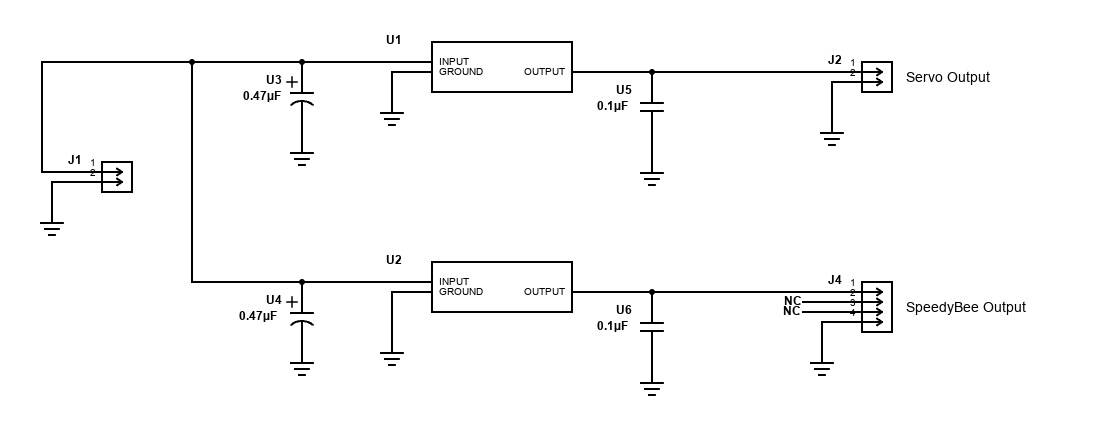
\includegraphics[height=6cm]{Voltage Regulator.png}
     \caption{12V-5V Voltage Regulator}
    \label{fig:Voltage Regulator}
\end{figure}
Fig. \ref{fig:Voltage Regulator} shows the schematic for the voltage regulator used to power both the servo motor and the Raspberry Pi. This circuit is centered around the L7805CV linear voltage regulator, which steps the 12V battery down to a stable 5V output and is capable of supplying up to 1.5A of current. The input and output capacitors are selected based on the recommendations provided in the datasheet to ensure optimal performance in DC applications.
\begin{figure}[H]
    \centering
    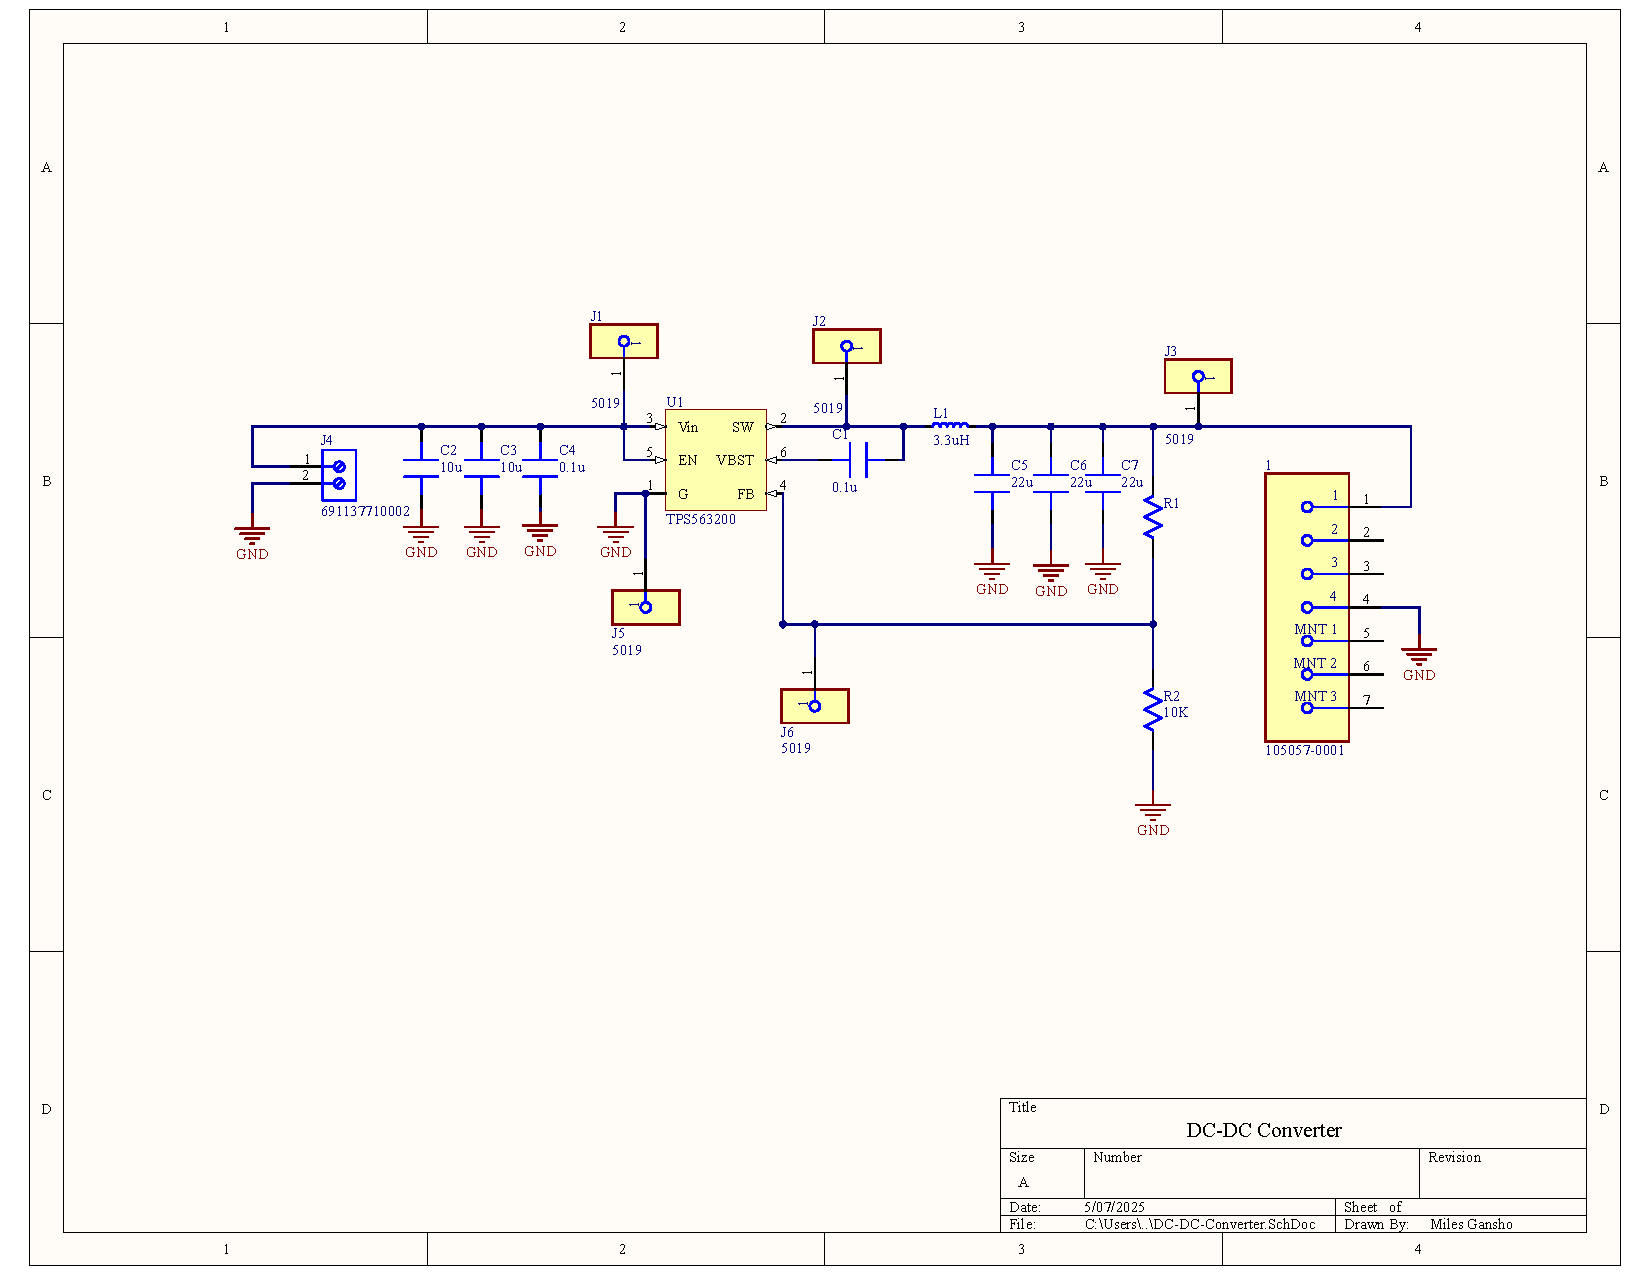
\includegraphics[height=7cm]{DC-DC converter.pdf}
     \caption{DC-DC converter}
    \label{fig:DC-DC Converter}
\end{figure}
Fig. \ref{fig:DC-DC Converter} is the second of our two designed circuits. This circuit also allows us to bring 12V down to a voltage we can use. However, the TPS563200 has a feedback on pin 4, which allows us to select a desired output voltage with the voltage divider constructed with R1 and R2. The output capacitors and inductors are selected based on datasheet recommendations for 5-7.5V outputs, and R1 is selected using the equation $V_{\text{out}} = 0.765 \times \left(1 + \frac{R_1}{R_2}\right)$. This chip also gives us an output current max of 3A, which is much higher than the voltage regulator, so better for larger loads.
\section{Simulation and Circuit Board Design}
Include URL links to any circuit simulation or PCB design files. You can store them on a folder in OneDrive. \textbf{Please add me as an owner so I can access the files after your account closes.}
\section{Physical Design}
\subsection{Frame and Flotation}
The ASV's frame is built from two 4" PVC pipes, each 30" long, mounted in parallel to provide flotation and structural support. A block of closed-cell EPS foam is secured beneath the pipes to improve buoyancy and overall water stability, as well as introducing some rigidity to the system. Closed-cell foam was required for underwater use, as open-cell foam would absorb water and lose buoyancy. The foam was cut to fit the frame and held in place with eight (1/4") bolts.

\subsection{Buoyancy Analysis}
The density of saltwater is approximately 1.025 kg/L, and we calculated the ASV's mass to be approximately 14.4 kg. With a 25\% safety factor, our target buoyancy is 18 kg. Buoyancy in kilograms is calculated by \(\text{Buoyancy} = \text{Weight of water displaced} \times \text{Volume of submerged object}\). For our geometry, the two PVC pipes displace 15.64 L and the EPS foam displaces 19.66 L, for a total volume of 35.3 L. With a saltwater density of 1.025 kg/liter, the total buoyancy of the ASV is \(1.025 \times 35.3 = 36.2 \) kg, well above our 18 kg requirement.

\subsection{Platform Structure}
A 24" wide platform sits atop the PVC pipes, consisting of two 1/8" MDF wooden struts for rigidity and a polycarbonate sheet for mounting structural components. Polycarbonate was chosen for its strength and durability, but it is very flexible; the MDF and EPS foam serve to stiffen the base while the polycarbonate provides a strong, flat mounting surface.

\subsection{Waterproof Enclosure and Solar Panel Mount}
A waterproof enclosure is mounted at the center of the platform to protect onboard systems. Above it, a \SI{100}{\watt} solar panel is held in place by four pairs of custom 3D-printed brackets. The brackets attach to the panel's corners and interface with 10"-long, (1/4") fiberglass composite rods seated in mating mounts. These brackets allow for easy removal of the solar panel for ease of transportation. The brackets proved strong enough to hold the panel, but future iterations could add captive set-screws to lock the rods in place rather than relying solely on friction and weight. An assembly view is shown in Figure~\ref{fig:solar-panel}.

\begin{figure}[htbp]
  \centering
  \includegraphics[width=0.4\linewidth]{"Solar_Panel_Assembly.png"}
  \caption{Solar panel assembly view.}
  \label{fig:solar-panel}
\end{figure}

\subsection{Motor Mounting and Flange Design}
The motor is mounted at the stern using a custom 3D-printed flange. The flange fits a 1" PVC shaft that connects the motor to the servo and keeps the shaft vertical during operation. To keep the motor in place, two 3D printed bushing were designed to fit the PVC shaft, which hold the motor at a constant depth. The bushing rotate above the flange, but the coefficient of friction between the two is low enough to allow the motor to rotate freely. This design choice ensures that the motor remains securely in place during operation, even in rough water conditions. The choice of a friction based bushing and flange system was chosen over a bearing system to reduce cost and complexity, as well as to allow for easy replacement of parts if needed.In Figure~\ref{fig:flange}, the servo sits in a recess to protect it from the elements, with its axis aligned to the PVC pipe so both rotate together.

\begin{figure}[htbp]
  \centering
  \includegraphics[width=0.4\linewidth]{"Flange_Assembly.png"}
  \caption{Flange assembly view.}
  \label{fig:flange}
\end{figure}

\subsection{3D-Printed Component Materials}
Material choice for 3D printed parts was given careful consideration to ensure the ASV is lightweight, low cost, but also resistant to wear. The 3D printed flange is made from ASA, a material known for its excellent UV resistance and mechanical properties. All other parts were made from PETG, which is a strong and durable material that maintains its structure underwater, making it suitable for the ASV's environment. The use of these materials ensures that the ASV can withstand the rigors of outdoor use while remaining lightweight and cost-effective. Structural parts were printed using 5 perimeters and 25\% gyroid infill, which provided a good balance of strength and weight, while also keeping costs relatively low. The entire project used under 750g of PETG, and around 250g of ASA, which can be purchased for around \$15. Further iterations could likely halve this number. Refer to the appendix for all isometric views of 3D printed parts.
\section{Electrical}

\subsection{Power Distribution}
The ASV is powered by two 12.8V 8Ah LiFePO4 batteries connected in parallel. A \SI{100}{\watt} solar panel mounted above the electronics enclosure outputs power to an MPPT controller, which continuously regulates the voltage and current to maximize the power output from the solar panel. The charge controller adjusts the variable DC that comes in from the solar panel to a constant voltage and current that is suitable for charging the batteries. The MPPT controller outputs the current through Anderson Powerpole connectors, which are tied into the circuit via a 12p junction terminal block, which distributes power to the rest of the system. The use of Anderson connectors allows for easy connection and disconnection of the solar panel. The batteries are connected with F2 spade connectors, also allowing for easy connection and disconnection.

Power is distributed through two voltage regulators that step the 12.8V battery voltage down to 5V. One converter supplies the SpeedyBee F405 V4 flight controller and GPS, and the other is dedicated to the servo motor. All components are placed inside a waterproof enclosure without mounting hardware. Initially, the voltage regulator was a buck converter on a PCB, but was replaced with a voltage regulator on a perfboard. The buck converter was not able to handle the current draw of the Speedybee, which caused it to overheat and fail. 

% Miles should write the section about the buck converters and the PCB design, but include a schematic of the protoboard

\subsection{Flight Controller and GPS}
\begin{figure}[H]
    \centering
    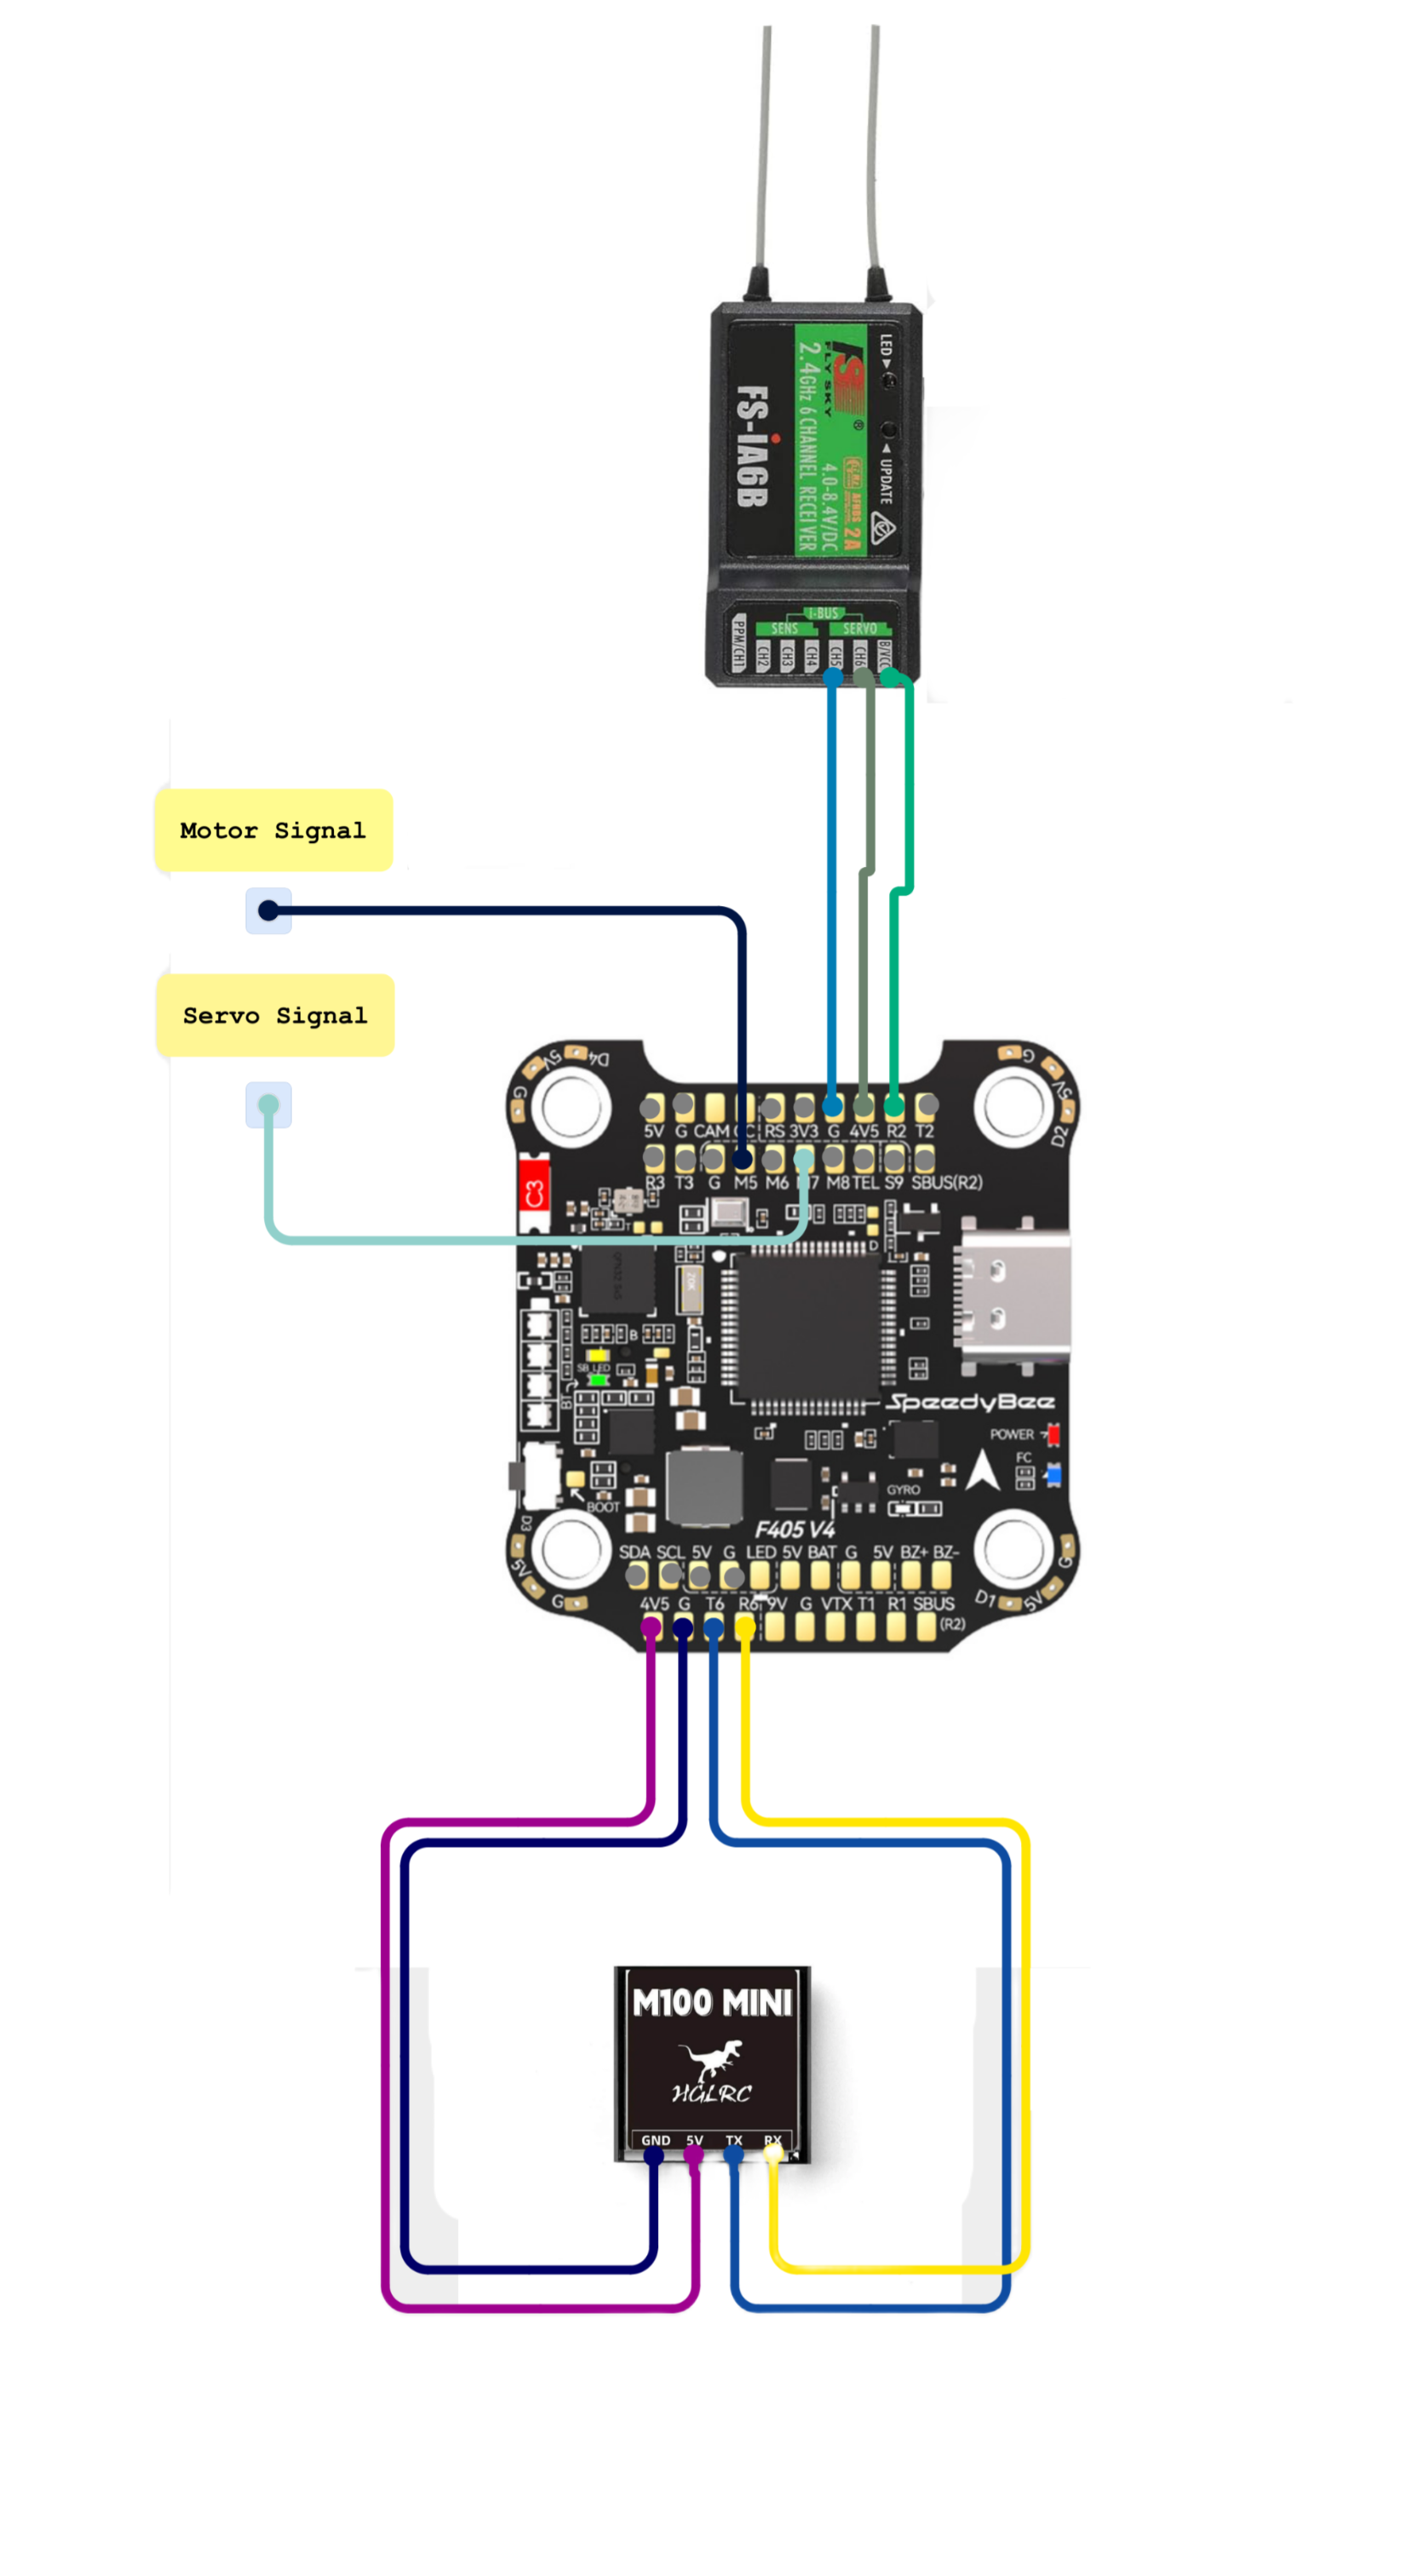
\includegraphics[height=10cm]{speedybee.png}
    \caption{Schematic of the SpeedyBee F405 V4 flight controller and its connections.}
    \label{fig:Speedybee}
\end{figure}

The SpeedyBee F405 V4 flight controller runs iNav firmware and handles both GPS waypoint navigation and motor control. It outputs PWM signals to the brushed DC motor and rudder servo and receives location data from a GPS module. The GPS is soldered directly to UART6 on the flight controller: TX from the GPS is connected to RX6, and RX from the GPS is connected to TX6. A FlySky FS-iA6B receiver is soldered directly to the RX2 pad on the flight controller for SBUS communication, enabling manual RC override when needed.

To generate a magnetic field, a 40 Hz sine wave is created by a prebuilt signal generator and passed through a power amplifier. The amplified signal drives a large copper coil wrapped around the boat’s structure, producing a low-frequency magnetic field detectable by submerged sensors.

The magnetic field \( B \) at the center of a circular coil is given by:

\begin{equation}
B = \frac{\mu_0 N I}{2R}
\label{eq:bfield}
\end{equation}

where:
\begin{itemize}
    \item \( \mu_0 = 4\pi \times 10^{-7} \, \text{T}\cdot\text{m/A} \) is the permeability of free space,
    \item \( N \) is the number of turns in the coil,
    \item \( I \) is the current through the coil,
    \item \( R \) is the radius of the coil.
\end{itemize}

This equation demonstrates that the magnetic field strength increases with more turns or higher current and decreases with a larger coil radius. The 40 Hz frequency was chosen to ensure good penetration through water with minimal signal loss, making it suitable for detection by submerged sensors.

All electrical connections are made using soldered wires. Power and signal lines are routed manually inside the enclosure. Signal and high-current paths are physically separated to minimize noise. Fuses are installed on the battery output lines to protect critical components from short circuits.

The electrical system is simple, modular, and designed for ease of repair and future upgrades. Components can be swapped or rewired without requiring full system disassembly.
\section{Coding}

In this section, we will include the programming aspects of our design.

% Commenting out all of the buoyancy calculations as they are not relevant to the final report.

% \subsection{Buoyancy Calculations}

% A crucial aspect of the RMS Titanic 2 autonomous surface vehicle is its ability to remain buoyant and stable while carrying all mission-critical components, including the electromagnetic coil of wire, electronic components, batteries, and solar panel. To ensure this, a comprehensive structural and buoyancy analysis was performed using a Python-based workflow.

% \subsubsection{Pipe and Material Specifications}

% The vessel's primary flotation is provided by two large-diameter PVC pipes, each with an inner diameter of 4 inches and a length of 30 inches.
% The density of polycarbonate (1210 kg/m$^3$) and seawater (1025 kg/m$^3$) were used as reference values for calculations.
% The mass of each PVC pipe was calculated using the manufacturer's specified weight per foot, converted to metric units for consistency.

% \subsubsection{Component Mass Budget}

% The total system weight includes all major components: electromagnetic coil (2.95 kg), servo, propulsion motor, LiFePO$_4$ battery, PVC housing, and a 6 kg solar panel.
% A 5\% contingency margin was added to account for mounting hardware, fasteners, and unforeseen additions.

% \subsubsection{The Analysis}
% The internal volume of each PVC pipe was computed and multiplied by the number of pipes to determine the total displaced volume.
% The buoyant force was calculated as the product of displaced seawater volume and seawater density.
% The total required buoyancy was set to the system's weight multiplied by a 1.25 safety factor, ensuring a 25\% margin for dynamic loads and environmental uncertainties.
% The difference between required buoyancy and the buoyancy provided by the PVC pipes determined the additional lift needed from closed-cell foam---we use Pink foam.

% \subsubsection{Foam Material Evaluation}

% Several foam options were considered, including marine-grade polyethylene, polyurethane, PVC foam, syntactic foam, and pink EPS foam- the latter being the most accessible and convenient whilst maintaining the properties required for floatation
% For each material, the required foam volume and example thickness (assuming a 30$\times$15 cm base area) were calculated, aiding in rapid material selection and prototyping.

% \subsubsection{Summary of Results}

% The analysis provided a clear breakdown of the vessel's mass, the buoyancy contribution of the PVC pipes, and the precise amount of additional foam required for safe operation.
% This approach allowed for iterative design, supporting quick assessment of the impact of component changes or material substitutions on vessel stability.
% The resulting design ensures that the ASV is robust and is capable of supporting all hardware without risk of sinking or instability, even under varying environmental conditions.
% This structural and buoyancy analysis was essential for validating the design of the RMS Titanic 2 platform, ensuring reliable operation during autonomous missions in coastal waters.

% \subsubsection{Python Code for Buoyancy Analysis}
% \begin{verbatim}
%     import math
    
%     # --- MATERIAL PROPERTIES ---
%     POLYCARB_DENSITY = 1210      # kg/m³, density of polycarbonate
%     SALTWATER_DENSITY = 1025     # kg/m³, typical density of seawater
    
%     # --- PIPE SPECIFICATIONS ---
%     NUM_PIPES = 2
%     INNER_DIAMETER_IN = 4.0      # Inner diameter in inches
%     LENGTH_IN = 30               # Length in inches
%     WEIGHT_PER_FOOT_PVC = 2.01
    
%     def in_to_m(inches):
%         """Convert inches to meters."""
%         return inches * 0.0254
    
%     # --- COMPONENT WEIGHTS (UPDATED WITH SOLAR PANEL) ---
%     components = {
%         'em_coil': 2.95,         # Electromagnetic coil
%         'servo': 0.068,          # Servo motor
%         'motor': 0.500,          # Propulsion motor
%         'battery': 1.80,         # LiFePO4 battery
%         'small_pvc': 0.227,      # PVC housing
%         'solar_panel': 6.00      # 6kg solar panel
%     }
    
%     # --- CALCULATE PIPE MASS USING INNER DIAMETER ---
%     inner_radius = in_to_m(INNER_DIAMETER_IN) / 2
%     length_m = in_to_m(LENGTH_IN)
%     single_pipe_volume = math.pi * (inner_radius ** 2) * length_m
%     total_pipe_volume = single_pipe_volume * NUM_PIPES
    
%     pipe_mass = (WEIGHT_PER_FOOT_PVC * LENGTH_IN / 12) # add lb to kg conversion
    
%     # --- TOTAL WEIGHT CALCULATION ---
%     component_sum = sum(components.values())
%     contingency = component_sum * 0.05  # 5% contingency
%     total_weight = component_sum + pipe_mass + contingency
    
%     # --- BUOYANCY ANALYSIS ---
%     displaced_volume = total_pipe_volume
%     buoyant_force = displaced_volume * SALTWATER_DENSITY
%     safety_margin = 1.25  # 25% safety factor
%     required_buoyancy = total_weight * safety_margin
%     required_foam = required_buoyancy - buoyant_force
    
%     # --- FOAM MATERIAL OPTIONS (INCLUDING PINK EPS FOAM) ---
%     # Buoyancy is equal to F= Rho * V * g;
%     # Weight of item m = density*v
%     # effective bouyant force Fb = F - g*m
    
%     foams = {
%         'Polyethylene': 0.90,    # Marine foam
%         'Polyurethane': 0.85,    # Marine foam
%         'PVC Foam': 0.52,        # Structural
%         'Syntactic Foam': 0.88,  # Deep water
%         'Pink EPS Foam': 0.98    #  lb/ft³ density (~32 kg/m³)2
%     }
    
%     print("[BUOYANCY ANALYSIS]")
%     print(f"Polycarbonate Pipe Mass: {pipe_mass:.2f} kg")
%     print(f"Total Vessel Weight: {total_weight:.2f} kg")
%     print(f"Pipe Buoyancy Contribution: {buoyant_force:.2f} kg")
%     print(f"Total Buoyancy Required: {required_buoyancy:.2f} kg")
%     print(f"Required Foam Buoyancy: {required_foam:.2f} kg\n")
    
%     print("[FOAM VOLUME REQUIREMENTS]")
%     print("Material         | Volume Needed (liters) | Example Thickness (cm)")
%     print("-----------------|------------------------|-----------------------")
    
%     for material, buoyancy in foams.items():
%         volume = required_foam / buoyancy if required_foam > 0 else 0
%         thickness = (volume * 1000) / (30 * 15)  # 30x15cm base area
%         print(f"{material:16} | {volume:8.1f}              | {thickness:5.1f}")
%     \end{lstlisting}
    
% \end{verbatim}

\subsection{Electromagnetic Coil Modeling and Magnetic Field Calculations}
A critical component of the RMS Titanic 2 system is the electromagnetic coil, which generates a low-frequency magnetic field for underwater detection and tracking. To optimize the coil design and predict its performance, a Python-based simulation was developed. This code calculates the electrical properties of a rectangular coil and simulates the resulting magnetic field at a specified observation point, using both analytical and numerical methods.

\subsubsection{Inductance and Electrical Properties Calculation}
The script first defines the coil geometry and material parameters, such as the number of turns ($N$), loop dimensions ($W$, $H$), wire diameter ($d$), and frequency ($f$). The inductance of the rectangular loop is calculated with a standard formula that accounts for the loop's physical dimensions and number of turns. The resistance is determined from the total wire length and resistivity, while the impedance is computed at the operating frequency. The magnetic moment, which sets the strength of the magnetic field, is also calculated as $m = NIA$.

\subsubsection{Magnetic Field Simulation}
The code then estimates the magnetic field at a specified observation point (typically 1 meter above the loop center) using two methods:

\begin{verbatim}
    # Magpylib Simulation (most accurate)
    if 'magpy' in globals():
        loop = magpy.current.Loop(
            current=N*I,
            diameter=np.sqrt(W**2 + H**2),
            position=(W/2, H/2, 0)
        )
        results['Magpylib'] = loop.getB(obs_point)
\end{verbatim}

\begin{verbatim}
    # Biot-Savart Numerical Integration
num_segments = 100  # Per side
dl = W/num_segments
B_bs = np.zeros(3)

for side in ['bottom', 'right', 'top', 'left']:
    for i in range(num_segments):
        if side == 'bottom':
            x = i*dl
            segment = np.array([x, 0, 0])
            dvec = np.array([dl, 0, 0])
        elif side == 'right':
            y = i*dl
            segment = np.array([W, y, 0])
            dvec = np.array([0, dl, 0])
        elif side == 'top':
            x = W - i*dl
            segment = np.array([x, H, 0])
            dvec = np.array([-dl, 0, 0])
        else:  # left
            y = H - i*dl
            segment = np.array([0, y, 0])
            dvec = np.array([0, -dl, 0])
        
        r = obs_point - (segment + dvec/2)
        r_mag = np.linalg.norm(r)
        B_bs += np.cross(dvec, r) / r_mag**3

B_bs *= (4*np.pi*1e-7) * N*I / (4*np.pi)
print("Biot-Savart B-field at observation point:", B_bs)

\end{verbatim}

\subsubsection{Output and Design Optimization}
The script prints all key electrical parameters, including magnetic moment, resistance, inductance, impedance, and required voltage for the desired current. It then outputs the magnetic field at the observation point for both calculation methods, supporting direct comparison and validation. If the magnetic moment is below a target threshold, the code suggests how to scale up current, turns, or area to achieve the desired performance.

\subsubsection{Engineering Value}
This modeling workflow enables rapid and accurate iteration of coil designs, balancing detection range, power consumption, and manufacturability. By integrating both analytical and numerical field calculations, the system ensures robust magnetic field generation tailored to the operational requirements of the RMS Titanic 2 platform.

\subsection{B-Field Coding}
Created a function that performs a comprehensive evaluation of square electromagnetic coils by analyzing various wire gauges and turn counts to identify feasible coil configurations that meet specified magnetic moment targets. Given a coil side length and a target magnetic moment range, the function calculates key electrical parameters including resistance, inductance, current requirements, and voltage ranges for each configuration. It utilizes a database of American Wire Gauge (AWG) specifications, incorporating wire diameter, resistance per meter, and maximum allowable current to ensure operational safety and efficiency. By iterating over practical turn counts and verifying current constraints, the analysis provides a set of viable coil designs optimized for magnetic performance and manufacturability. This systematic approach facilitates informed decision-making in coil design, balancing physical dimensions and electrical characteristics to achieve desired magnetic moments within practical power and thermal limits. We ultimately did not use this- but we mention this here as something we had tried.

\begin{equation}
V=\oint \overrightarrow{E}\cdot d\overrightarrow{l}  
\label{MyEquation}
\end{equation}

\subsection{iNav Configuration}

The SpeedyBee F405 V4 flight controller was flashed with iNav 7 firmware to enable GPS-based return-to-home (RTH) functionality and manual control. iNav 7 was selected because of its improved support for surface vehicles, enhanced GPS navigation features, and full compatibility with the SpeedyBee F405 V4 without requiring custom firmware builds.

\subsubsection*{Mixer Modifications}

By default, iNav's boat mixer uses differential thrust with two motors for steering. Since our ASV uses a single brushed DC motor for propulsion and a rudder servo for steering, this default configuration was unsuitable.

To support our hardware, we modified the mixer setup in \texttt{mixer.c} to map throttle directly to Motor 0 and yaw to Servo 0. Pitch and roll mixing were disabled, as they are unnecessary for surface operation. This allowed the boat to steer using the rudder while maintaining forward propulsion with the single motor.

\subsubsection*{Firmware Configuration Changes}

Several key settings were configured using the iNav Configurator and CLI to support manual control and GPS-assisted return-to-home:

\begin{itemize}
    \item \textbf{Ports:}
    \begin{itemize}
        \item UART6 configured for GPS (UBlox protocol)
        \item UART2 configured for SBUS receiver (FlySky FS-iA6B)
    \end{itemize}
    \item \textbf{Failsafe:} Configured to trigger Return-to-Home (RTH) on signal loss.
    \item \textbf{Flight Modes:} Enabled MANUAL, ANGLE, and RTH. AUTO mode was left disabled.
    \item \textbf{Arming:} Manual arming allowed when GPS lock is acquired.
    \item \textbf{PID Tuning:} Pitch and roll control disabled; yaw PID tuned for surface steering only.
\end{itemize}

Example CLI commands used:

\begin{lstlisting}
mixer load boat
set gps_provider = UBLOX
set gps_auto_config = ON
set gps_auto_baud = ON
set serialrx_provider = SBUS
set failsafe_procedure = RTH
set nav_rth_allow_landing = OFF
save
\end{lstlisting}

\subsubsection*{Source Code Adjustments}

The full iNav firmware was not rewritten, but minor modifications were made to the mixer definitions in \texttt{mixer.c} to support single-motor with rudder control. No other firmware files were changed. iNav’s official repository was used as the base.

\subsubsection*{Reproduction Instructions}

To reproduce this firmware setup:

\begin{enumerate}
    \item Clone the official iNav firmware repository:
    \begin{lstlisting}
git clone https://github.com/iNavFlight/inav.git
cd inav
    \end{lstlisting}

    
    \item Modify \texttt{src/main/mixer/mixer.c} to implement a single-motor and rudder mixer by:
    \begin{itemize}
        \item \textbf{Disable pitch and roll mixing} by setting these inputs to zero in the \texttt{mixTable()} function:
        \begin{lstlisting}[language=C]
            input[ROLL] = 0;
            input[PITCH] = 0;
        \end{lstlisting}

        \item \textbf{Map throttle to Motor 0 only} by replacing the motor loop with:
        \begin{lstlisting}[language=C]
            for (int i = 0; i < motorCount; i++) {
                if (i == 0) {
                    motor[i] = mixerThrottleCommand;
                } else {
                    motor[i] = motorZeroCommand;
                }
            }
        \end{lstlisting}

        \item \textbf{Map yaw to Servo 0} by ensuring yaw control is configured in the servo mixer or output settings, instead of applying yaw to the motor mixer.
    \end{itemize}


    \item Build the firmware following iNav's official build instructions.

    \item Flash the compiled firmware to the SpeedyBee F405 V4.

    \item Apply the CLI configuration listed above.

    \item Test GPS lock, receiver input, motor output, rudder control, and Return-to-Home functionality before deployment.
\end{enumerate}

\subsubsection*{Summary}

These modifications allowed the ASV to operate with stable manual control and GPS-assisted return-to-home, while disabling unnecessary flight-specific features.

\bigskip

The complete project repository, including design documentation, hardware details, software configuration, and source code references, is available at:

\begin{center}
\url{https://github.com/grgao/boat/tree/main/ECE%20455_Report}
\end{center}
\section{Operating Instructions}

Follow these steps to safely operate the Autonomous Surface Vehicle (ASV):

\begin{enumerate}
    \item \textbf{Power On:}
    \begin{itemize}
        \item Ensure the batteries are charged. The solar panel provides slow passive charging and should not be relied on for full charge.
        \item Inside the electronics enclosure, connect the battery wires. Each lead is clearly labeled for polarity—connect positive to positive and negative to negative.
        \item Verify that LEDs on the flight controller (SpeedyBee F405 V4) illuminate, indicating power to the system.
    \end{itemize}

    \item \textbf{System Initialization:}
    \begin{itemize}
        \item Wait a few seconds for the flight controller to initialize.
        \item Confirm GPS lock. The GPS module's LED (typically solid or blinking depending on model) indicates satellite connection.
    \end{itemize}

    \item \textbf{Manual Control (Optional):}
    \begin{itemize}
        \item Turn on the FlySky transmitter. Ensure the receiver on the ASV is powered and paired.
        \item When connected, you can use the transmitter to manually control throttle and rudder. This is useful for testing or override.
        \item Manual control is not required for autonomous operation but is available at any time.
    \end{itemize}

    \item \textbf{Autonomous Mission Launch:}
    \begin{itemize}
        \item Use iNav Configurator to upload or verify the waypoint mission.
        \item Use iNav Configurator to verify basic telemetry such as GPS status, battery voltage, and input channel readings.
        \item Confirm that all connections are secure and components are functioning.
        \item Arm the vehicle using the transmitter or iNav interface. The motor should begin spinning, and the boat can now be manually operated or left to drift as designed.
    \end{itemize}

    \item \textbf{Magnetic Field Activation:}
    \begin{itemize}
        \item The signal generator automatically powers on with the system and begins outputting a 40 Hz sine wave.
        \item The output is amplified and fed to the coil. If needed, use a clamp meter to verify that current is flowing.
    \end{itemize}

    \item \textbf{Monitoring:}
    \begin{itemize}
        \item Observe the ASV visually or via iNav telemetry if connected.
        \item Monitor GPS LED status and waypoint progress to confirm correct operation.
    \end{itemize}

    \item \textbf{Return to Home and Shutdown:}
    \begin{itemize}
        \item Use the transmitter or iNav to switch to “Return to Home” mode. The ASV will autonomously return to its starting location.
        \item Once the vehicle has returned and stopped moving, disarm it using iNav or the transmitter.
        \item Disconnect the battery by separating the labeled leads.
        \item Verify that all indicator LEDs are off and reseal the electronics enclosure to maintain waterproofing.
    \end{itemize}
\end{enumerate}

Before each deployment, double-check polarity labels, confirm dry connections, and verify GPS and flight controller status.

\section{Troubleshooting and Testing}
During our project, we encountered various challenges that required creative problem-solving to keep things moving. Whether it was soldering mistakes, power-related issues, or flaws in the physical design, no prototype is perfect on the first try. This section outlines the key problems we faced during development, how we addressed them, and what test we performed on the prototypes. this section will also discuss things we couldn't get working exactly how we wanted and what steps should be taken to fix them.
\subsection{PCB and Power}
When designing the PCB, we considered several chip options but ultimately settled on the TPS563200. This chip was selected using the WEBENCH Power Designer. This software allows you to pick an input voltage, desired output voltage, and current, and then generate possible chips and schematics. This allowed us to generate some simulation files like the one seen in Fig. \ref{fig:Vout}. This shows a simulated start-up using this chip. R1 is selected so that \(V_{\text{out}}\) is 5V, and as you can see from the simulation, that is exactly what we got.
\begin{figure}[H]
    \centering
    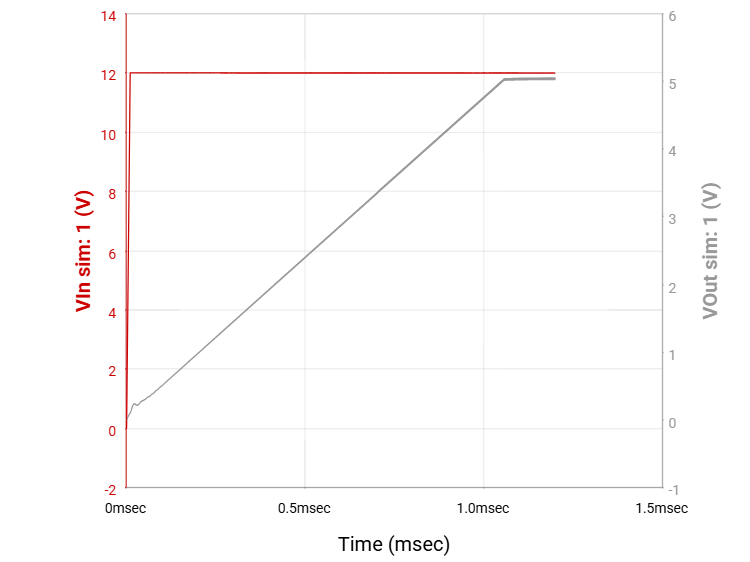
\includegraphics[height=6cm]{Vout_chart.png}
     \caption{Simulated Start up for the TPS563200}
    \label{fig:Vout}
\end{figure}
The DC-DC converter PCB was one of the many problems we had to overcome. The main issue was that the PCB successfully worked at larger loads($20~\Omega$), which drew around 0.25 amps. However, when we decreased the load to $3.5~\Omega$, drawing around 1.5A, the chip would burn out. After looking at potential issues ranging from lack of inrush current protection, voltage spikes, etc., the actual issue turned out to be the lack of a \(V_{\text{out}}\) copper pour between the inductor and output capacitors. The copper pour allows for good heat dissipation within the circuit, and since we didn't have any, the chip would overheat at low loads. We tried a couple of quick fixes like soldering more connections between the output capacitors and the inductor or increasing output capacitance. These solutions would hold the voltage for a little longer, up to around one minute, but ultimately they would burn up. So we switched to a voltage regulator, which, although it has a lower output current, was still sufficient to operate the servo and power the SpeedyBee. A long-term fix for using a DC-DC converter would be to redesign the PCB with a \(V_{\text{out}}\) pour to allow for better heat dissipation.
\subsection{Motor Operation and Grounding}
The main motor used for propulsion was one of the first challenges we had to overcome when dealing with the construction of our ASV. We purchased our motor with an ESC already included, which allowed us to control the motor with just power and a PWM signal wire. However, when trying to power our motor, we had trouble with the initial start. The way to fix this issue was to make sure everything had a common ground. Soldering the Raspberry Pi, SpeedyBee, and battery grounds together ensures no ground is floating, and we can get a clean signal to our motor from the SpeedyBee. In the future, a custom PCB with a shared ground rail would be the most effective way to ensure all grounds are the same, and save the most amount of space instead of soldering all the grounds together. 
\subsection{Physical Construction and Design}
Physical construction came with many unforeseen challenges, especially since the majority of our group specialized in electrical design and coding. One of the main issues we ran into was selecting what kind of material to make the base of our ASV with. The original plan was to make the base of the ASV out of acrylic. This would provide a lightweight base and allow us to laser cut or drill through it so we could attach things like the motor flange and our coil. However, when constructing our ASV, the acrylic sheet snapped under the tension of our coil while we were trying to drill the 1" hole for the motor connection. This made us switch to polycarbonate, which is slightly more flexible but is easier to drill through and cut. We also added MDF wood to give the base of the ASV a little more strength. In the future, teams should try and look to replace the MDF wood with something a little more secure and lightweight. Also, if future groups decide to go back to acrylic, the base case to cut through it is to laser cut all the holes for better precision.  
\section{Testing and Experiments}
Here you can talk about your experimental results and include plots of any relevant data. The plots should be of professional quality. Use Python, MATLAB, or OriginLab. Excel in the engineering world is not professional. 


\section{Future Work}

There is a considerable amount of work that can be done to improve the ASV, as this was a prototype. During our design phase, we were limited by time and budget constraints, but future teams can build on our work to create a more robust and effective systems, especially if they can learn from our mistakes. The following sections will discuss some of the most important areas for improvement, including physical design, electronics, software, and testing. 

\subsection{Physical Design}

Several improvements to our prototype's mechanical structure should be considered for future ASV iterations:
\begin{itemize}
  \item \textbf{Optimized Part Geometry for Weight \& Strength:}  
    Our 3D-printed components were designed under tight time constraints and saw only a few iterations. If budget allows, future teams should perform wear tests on the 3D printed parts to see where they fail, and then redesign to optimize for weight and strength. There were a few prints where it was clear that the part was acceptable, but could use an easy redesign to improve the functionality. For example, the flange was one piece, but if it was split into two pieces, it would be easier to print and assemble.
  \item \textbf{Bracket Offset \& Mounting Security:}  
    The solar panel (27.5" wide) extended beyond our only one of four bolts could engage, leading to instability. This could be solved by redesigning the bracket geometry or increasing the offset distance to ensure all fasteners seat properly. Additionally, the panel support rods currently rely on friction and panel weight to stay in their mounts. Introduce captive set-screws or spring-loaded clips in each bracket to mechanically lock the rods in place, preventing slippage under harsh conditions    
  \item \textbf{Platform Material Stiffness:}  
    Our polycarbonate sheet platform flexed under load. A stiffer base, such as treated wood, aluminum, or even a thicker sheet of polycarbonate, would reduce deflection, improve stability, and better support mounted components.
  \item \textbf{Waterproofing at Fastener Joints:}  
    To preserve disassembly ease, we avoided epoxy and ran bolts through PVC fixtures, which allowed water ingress. Future designs should apply marine epoxy or silicone sealant at critical joints, or employ O-ring-sealed fastener assemblies, to balance rigidity, waterproofing, and maintainability. The mounting holes may have to be redesigned to accommodate this, as the current design doesn't allow for easy disassembly after the epoxy is applied. If the ASV is to fit in a suitcase, then the easy assembly and disassembly of the ASV is a critical component of the next design phase. 
\end{itemize}

\subsection{Electronics}

Several lessons from our prototype's wiring and power distribution should guide future iterations:
\begin{itemize}
  \item \textbf{Modular Motor Connections:} 
    Our motors were hard-wired via fully soldered leads, making removal and replacement cumbersome. Future designs should employ waterproof, keyed connectors inside the electrical box to allow rapid motor swap-outs for maintenance or upgrades without desoldering. We used some Anderson Powerpole connectors for the MPPT connections, but they were a bit cumbersome to use, as well as not waterproof. 
  \item \textbf{Overcurrent \& Reverse Polarity Safeguards:} 
    We lacked fusing or electronic breakers on our high-current rails. Future designs should include appropriately rated fuses or resettable circuit breakers on each major branch (motor, batteries, electronics) to isolate faults and protect wiring and components.
    Additionally, during our demo, the battery pack was accidentally connected backwards, risking damage to electronics and breaking our ESC. Future designs should incorporate reverse-polarity protection—using an ideal-diode IC or MOSFET-based blocker in the main power feed—to automatically guard against destructive reverse connections and prevent user error.
  \item \textbf{Power Distribution Board (PDB):} 
    Our prototype relied on wiring into a terminal junction bock, which increased bulk cabling and complicated troubleshooting. Future designs should use a custom PDB with integrated connectors, breakers, and status LEDs, with silk-screened labels marking each output (e.g.\ “Motor,” “MPPT,” “Servo”). A dedicated PCB, designed from the ground up, could consolidate off-the-shelf power components (amplifiers, signal generators, buck converters) into a single compact board, significantly reducing wiring complexity and system footprint.
  \item \textbf{Outputting Sine Wave from SpeedyBee:}
    If the SpeedyBee is to be used for a future iteration, it would be beneficial to test if it is possible to output the sine wave directly from the onboard ESC. The ESC outputs a 3 phase voltage to drive a brushless motor, and if the frequency of the sine wave is low enough, it may be possible to use the ESC to drive the coil directly. This would reduce the number of components needed and simplify the design. However, if an entire PCB were to be made, then this step is not as necessary. Additionally, if more motors were to be purchased, buying brushless motors would be cheaper than motors with a built in ESC, as the SpeedyBee fv405 V4 stack comes with an ESC to drive these motors. 
  \item \textbf{Adding Second Coil to Improve GPS:}
    The GPS module was subject to interference from the coil, which made it difficult to get a good GPS signal. With a second coil emitting a magnetic field in the opposite direction, it would be possible to cancel out the interference from the first coil. This would allow for a much better GPS signal. The second coil would need to be placed at a distance from the first coil, and it could be in series with the first coil and just wound in the opposite direction. Placing the coils in series ensures that the coils are in phase with each other, but the output would cancel out the field from the first coil.
\end{itemize}
    
\subsection{Software}
Our iNav configuration was a basic setup, and future teams should consider utilizing the software ArduPilot, which is a more robust but complex system.
\begin{itemize}
  \item \textbf{Space Filling Curve Algorithm:} 
    We used simple waypoint-following, but future teams should consider implementing a space-filling curve algorithm to optimize the ASV's path. This would allow the ASV to cover more area in less time, improving efficiency and data collection. The current system requires users to manually set waypoints, which is time-consuming and inefficient. A space-filling curve algorithm would allow the ASV to autonomously navigate a given area, reducing the need for manual waypoint setting and improving the user's experience.
\end{itemize}
\subsection{Testing}

Testing was one of our biggest challenges, as we did not get enough time to test the ASV in the water, because by the time we were ready to test, we realized that it was likely not worth the difficulty of waterproofing the bolt connections, which would also make the handoff of the project significantly more difficult. The following are some suggestions for future teams to consider when testing the ASV:
\begin{itemize}
  \item \textbf{Testing the Coil:} 
    We were unable to test the coil in the water to ensure that it actually reached the depth we calculated. Above the water the coil was able to produce a magnetic field, but our simulations showed that the field would be detectable at a depth of 80 feet underwater. Future teams should consider a methodology for testing the coil, even if it is not in the water.
  \item \textbf{Testing in a Real Environment:} 
    Future teams should consider testing the ASV in a controlled environment, such as a pool, before taking it out into somewhere like Lake Mendota. This would allow for easier troubleshooting and debugging of the system, as well as providing a safer environment for testing. Testing in a large lake would be beneficial to see how the ASV performs in a real environment, but it would be much more difficult to troubleshoot and debug the system.
    
\end{itemize}


\bibliographystyle{IEEEtran}
\bibliography{ref}



% ------------------------------------------------------------------------------
% End document
% ------------------------------------------------------------------------------
\end{document}